\documentclass[tikz,border=8pt]{standalone}
\usetikzlibrary{arrows.meta,positioning,automata,calc}

\begin{document}
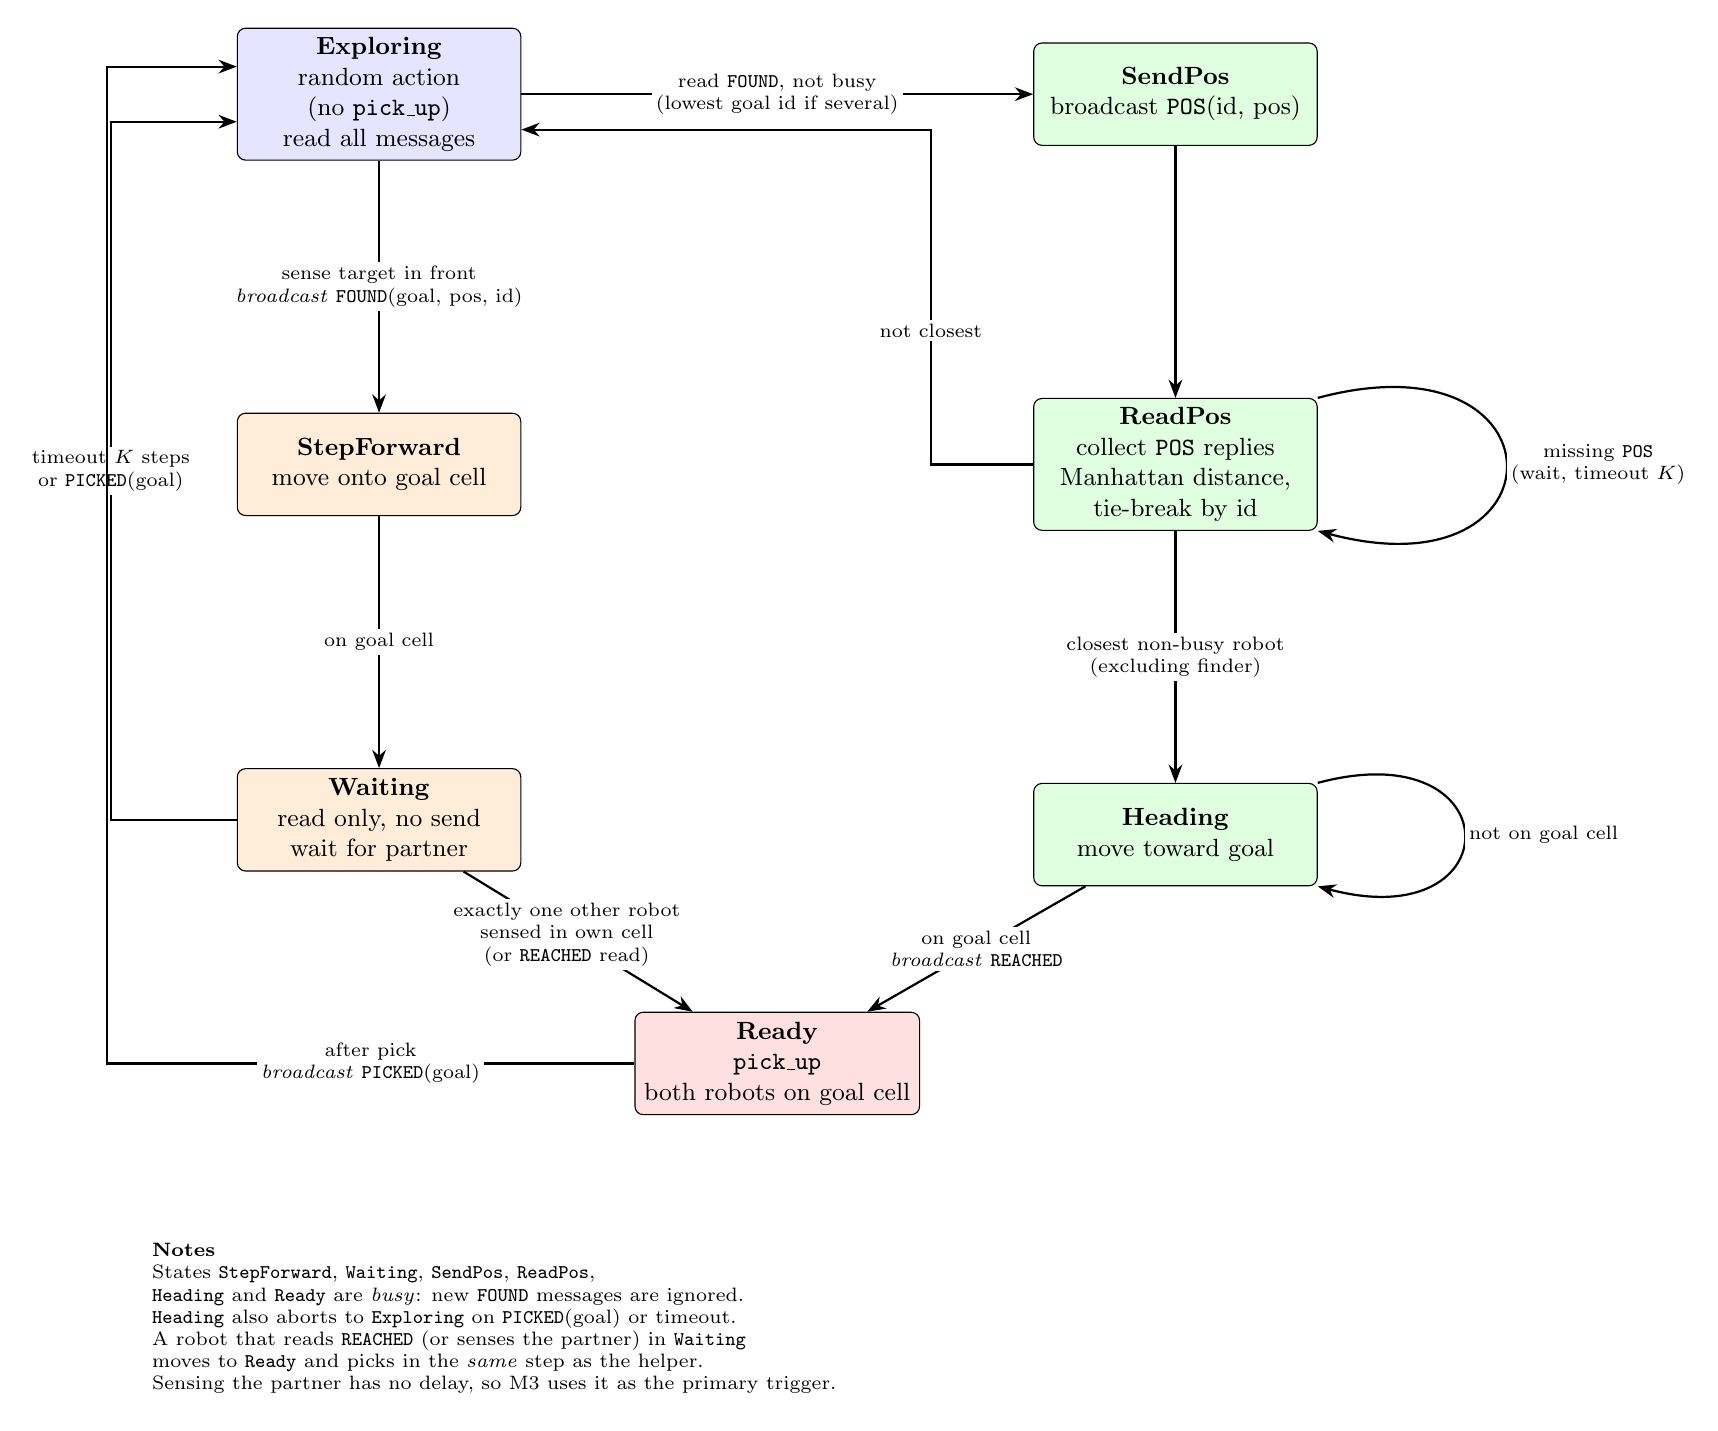
\begin{tikzpicture}[
    >=Stealth,
    node distance=3.2cm and 6.5cm,
    state/.style={draw, rounded corners=3pt, minimum width=3.6cm,
                  minimum height=1.3cm, align=center, font=\small},
    explore/.style={state, fill=blue!10},
    finder/.style={state, fill=orange!15},
    helper/.style={state, fill=green!12},
    shared/.style={state, fill=red!12},
    tr/.style={->, thick},
    lbl/.style={font=\scriptsize, align=center, fill=white, inner sep=1.5pt},
    note/.style={font=\scriptsize, align=left}
]

% ---------- states ----------
\node[explore] (explore) {\textbf{Exploring}\\
  random action\\(no \texttt{pick\_up})\\read all messages};

\node[finder, below=of explore]  (step) {\textbf{StepForward}\\
  move onto goal cell};
\node[finder, below=of step]     (wait) {\textbf{Waiting}\\
  read only, no send\\wait for partner};

\node[helper, right=of explore]  (sendpos) {\textbf{SendPos}\\
  broadcast \texttt{POS}(id, pos)};
\node[helper, below=of sendpos]  (rank) {\textbf{ReadPos}\\
  collect \texttt{POS} replies\\Manhattan distance,\\tie-break by id};
\node[helper, below=of rank]     (head) {\textbf{Heading}\\
  move toward goal};

\node[shared] (ready) at ($(wait)!0.5!(head)+(0,-3.0)$) {\textbf{Ready}\\
  \texttt{pick\_up}\\both robots on goal cell};

% ---------- finder path ----------
\draw[tr] (explore) -- node[lbl,pos=.5]{sense target in front\\
  \textit{broadcast} \texttt{FOUND}(goal, pos, id)} (step);
\draw[tr] (step) -- node[lbl]{on goal cell} (wait);
\draw[tr] (wait) -- node[lbl,pos=.45]{exactly one other robot\\sensed in own cell\\(or \texttt{REACHED} read)} (ready);
\draw[tr] (wait.west) -- ++(-1.6,0) |- node[lbl,pos=.25]{timeout $K$ steps\\or \texttt{PICKED}(goal)} ($(explore.west)+(0,-0.35)$);

% ---------- helper path ----------
\draw[tr] (explore) -- node[lbl,pos=.5]{read \texttt{FOUND}, not busy\\
  (lowest goal id if several)} (sendpos);
\draw[tr] (sendpos) -- (rank);
\draw[tr] (rank) -- node[lbl]{closest non-busy robot\\(excluding finder)} (head);
\draw[tr] (rank.west) -- ++(-1.3,0) |- node[lbl,pos=.2]{not closest} ($(explore.east)+(0,-0.45)$);
\draw[tr] (rank.north east) to[loop right, looseness=5] node[lbl,right]{missing \texttt{POS}\\(wait, timeout $K$)} (rank.south east);
\draw[tr] (head.north east) to[loop right, looseness=5] node[lbl,right]{not on goal cell} (head.south east);
\draw[tr] (head) -- node[lbl,pos=.5]{on goal cell\\\textit{broadcast} \texttt{REACHED}} (ready);

% ---------- common exits ----------
\draw[tr] (ready.west) -- node[lbl,pos=.5]{after pick\\\textit{broadcast} \texttt{PICKED}(goal)} ++(-6.7,0) |- ($(explore.west)+(0,0.35)$);

% ---------- legend ----------
\node[note, anchor=north west] at ($(wait.south west)+(-1.2,-4.6)$) {%
  \textbf{Notes}\\
  States \texttt{StepForward}, \texttt{Waiting}, \texttt{SendPos}, \texttt{ReadPos},\\
  \texttt{Heading} and \texttt{Ready} are \emph{busy}: new \texttt{FOUND} messages are ignored.\\
  \texttt{Heading} also aborts to \texttt{Exploring} on \texttt{PICKED}(goal) or timeout.\\
  A robot that reads \texttt{REACHED} (or senses the partner) in \texttt{Waiting}\\
  moves to \texttt{Ready} and picks in the \emph{same} step as the helper.\\
  Sensing the partner has no delay, so M3 uses it as the primary trigger.};
\end{tikzpicture}
\end{document}
